\documentclass[a4paper]{article}

%% Language and font encodings
\usepackage[english]{babel}
\usepackage[utf8x]{inputenc}
\usepackage[T1]{fontenc}

%% Sets page size and margins
\usepackage[a4paper,top=3cm,bottom=2cm,left=3cm,right=3cm,marginparwidth=1.75cm]{geometry}

%% Useful packages
\usepackage{amsmath}
\usepackage{graphicx}
\usepackage[colorinlistoftodos]{todonotes}
\usepackage[colorlinks=true, allcolors=blue]{hyperref}

\title{4th Paper: Optimal Grid Design in Operating Models: Work smarter, not harder}
\author{Iago Mosqueira, Rishi Sharma, Laurie Kell, Toshihide  Kitakado}

\begin{document}
\maketitle

\begin{abstract}

... 

\end{abstract}

\section*{Outline}

\begin{itemize}
\item Pose the hypothesis that the performance of Model Based MPs depend on the Production Function and that empirical MPs depend on the nature of the time series.
\item Summarise the ALBIO grid, WRT the expected dynamics and the nature of the time series.
\item Throw in some non-stationary, i.e. based on Hjort, Cury, Bjornstat, and ...
\item Conduct MSE and use regression trees to identify what are the important uncertainties to resolve in order to meet the four management objectives of safety, status, yield and stability
\item Is it the factors modelled by the grid scenarios or the emergent properties? this has important consequences for conditioning OMs. 
\end{itemize}

\section{Introduction}

When conducting Management Strategy Evaluation (MSE) Operating Models (OMs) are commonly \citep[][]{} conditioned using stock assessment models, using a grid design to model structural uncertainty and data conflicts. For example the Indian Ocean Albacore MSE used Stock Synthesis to develop scenarios based on parameters that are difficult to estimate (i.e. M, steepness, and selectivity) and the relative weightings of the indices of abundance and the length data. The choice of OMs is important as the \textit{best} Management Procedure is determined by the choice of hypotheses represented by the OM.
It is often not possible, however, to assign plausibility to the different scenarios, therefore the rationale for the grid design is of fundamental importance.

MSE’s often use complicated grid based platforms to test alternative states of nature (e.g. CCSBT, Hillary et al. 2016 ). This was the case in initial development for Albacore in the Indian Ocean (Mosqueira and Sharma 2014 IOTC 2014-WPM 05) based on the Synthesis Assessment (Hoyle et. al. 2014). In that case 720 models were examined as the basis of the operating model. However, in the case of the Atlantic (Kell et. al. 2016), a much finer operating model structure was used (10 models) conditioned on the MultiFan Assessment (Anon 2012).  Thus, a whole range of approaches is available in the literature (Punt et. al. 2014) and we would examine if a full grid approach is relevant, or something simpler could work. 

The objective of this work is to first explore the grid structure used for Indian Ocean albacore, i.e. to identify the characteristics that will impact the performance of the MPs being tested. There are two main properties of the OM in this regard, i.e. the expected dynamics as represented by the production function, and the nature of the time series.

Therefore we first summarise the OM scenarios, before conducting an MSE for model based and empirical control rules. 

\section{Material and Methods}
\subsection{Material}

\begin{itemize}
    \item Use ALBIO OM
\end{itemize}

\section{Methods}

\begin{itemize}
    \item Summarise production functions and reference points wrt grid
    \item Summarise time series, i.e. process error wrt grid
    \item Run MP based on biomass dynamic model 
    \item Run MP based on empirical Rule
    \item Use regression tree to identify which rule performs best.
    \item Identify the effect of uncertainty on performance.
\end{itemize}

\section{Results}

\textbf{Figure \ref{fig:kobe}} Kobe phase plot for the full grid.

\textbf{Figure \ref{fig:majuro}} Majuro  plot for the full grid.

\textbf{Figure \ref{fig:ssb}} Time series of SSB for full grid.

\textbf{Figure \ref{fig:grid}} Summary of grid scenarios.

\textbf{Figure \ref{fig:pf}} Production functions for the full grid.

\textbf{Figure \ref{fig:pe}} Process error for the full grid.


\bibliographystyle{alpha}
\bibliography{sample}

\section{Figures}
\newpage\clearpage

\begin{figure}
\centering
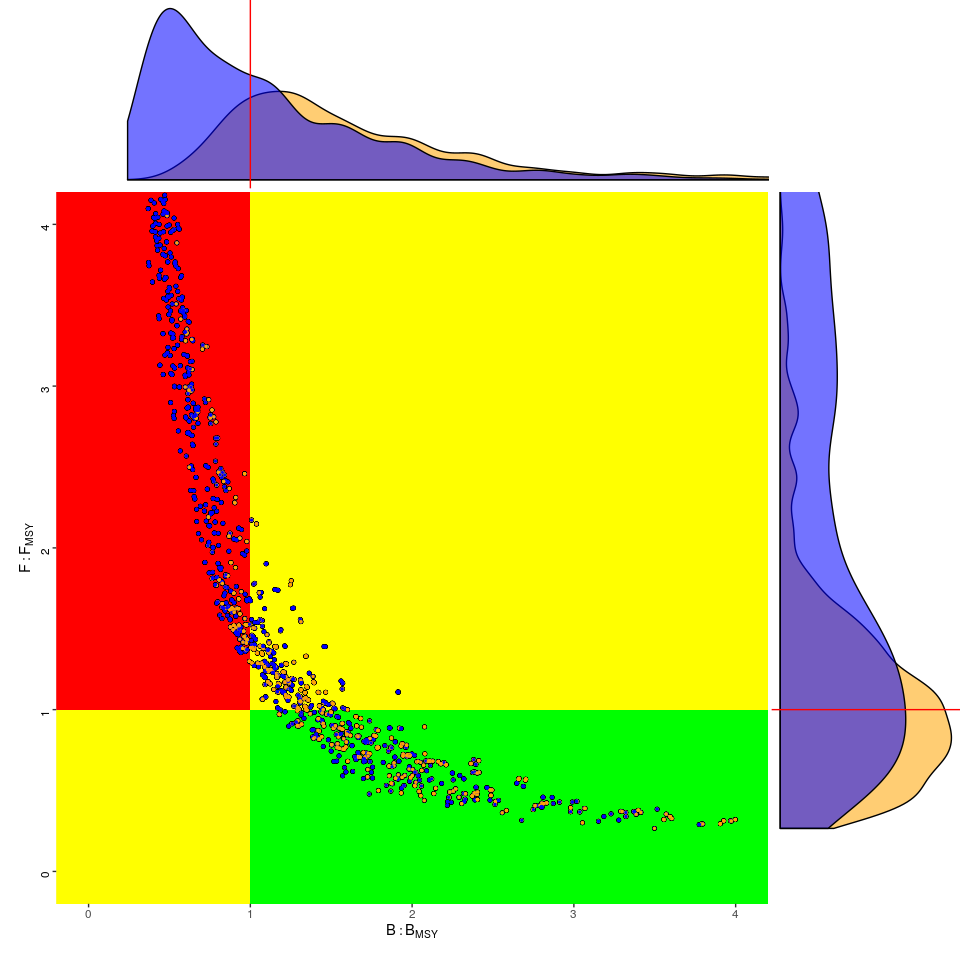
\includegraphics[width=0.75\textwidth]{alb-kobe1-1.png}
\caption{\label{fig:kobe} Kobe phase plot for the full grid.}
\end{figure}

\begin{figure}[ht]
\centering
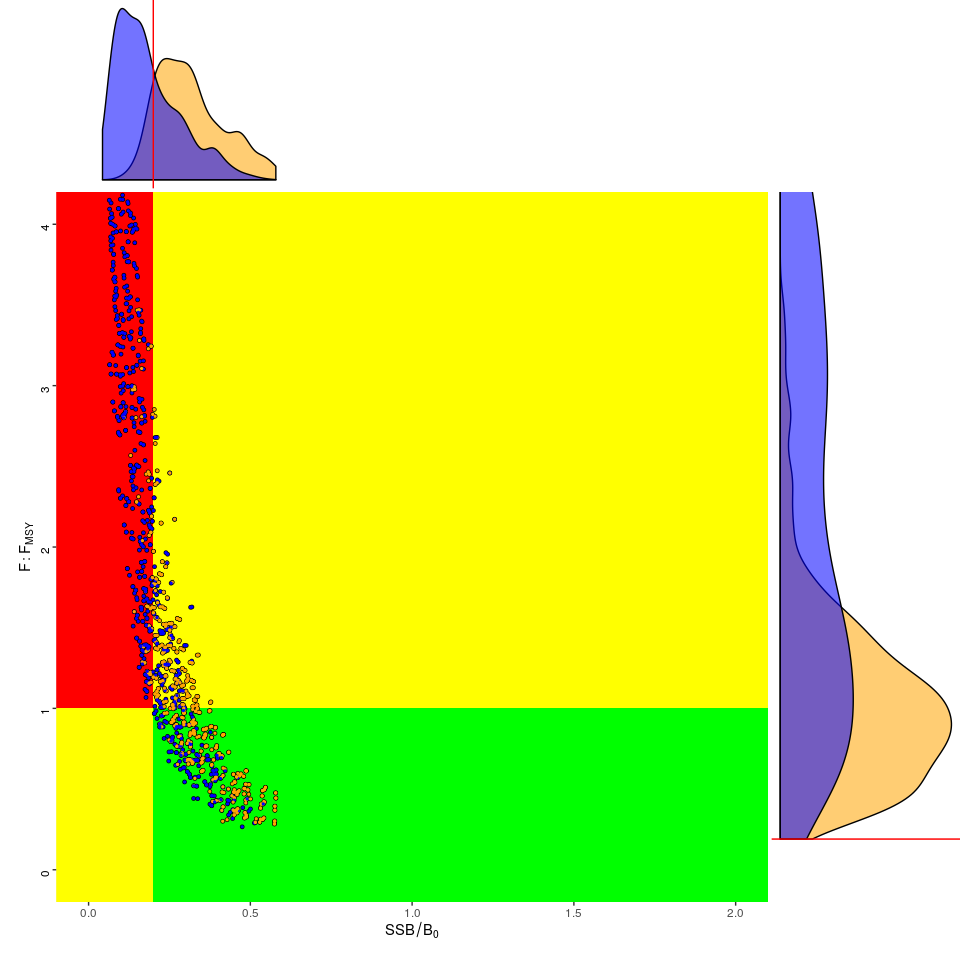
\includegraphics[width=0.75\textwidth]{alb-majuro1-1.png}
\caption{\label{fig:majuro} Majuro  plot for the full grid.}
\end{figure}

\begin{figure}[ht!]
\centering
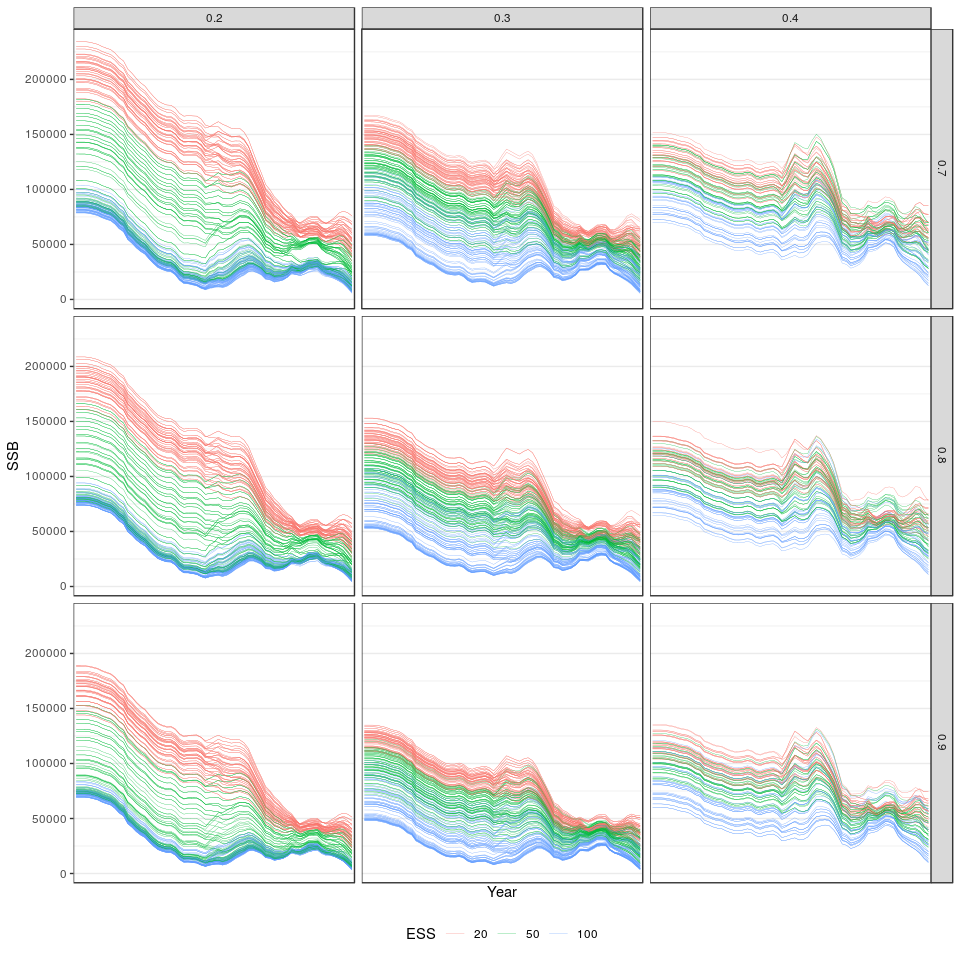
\includegraphics[width=0.75\textwidth]{alb-ssb-1.png}
\caption{\label{fig:ssb} Time series of SSB for full grid.}
\end{figure}

\begin{figure}[ht!]
\centering
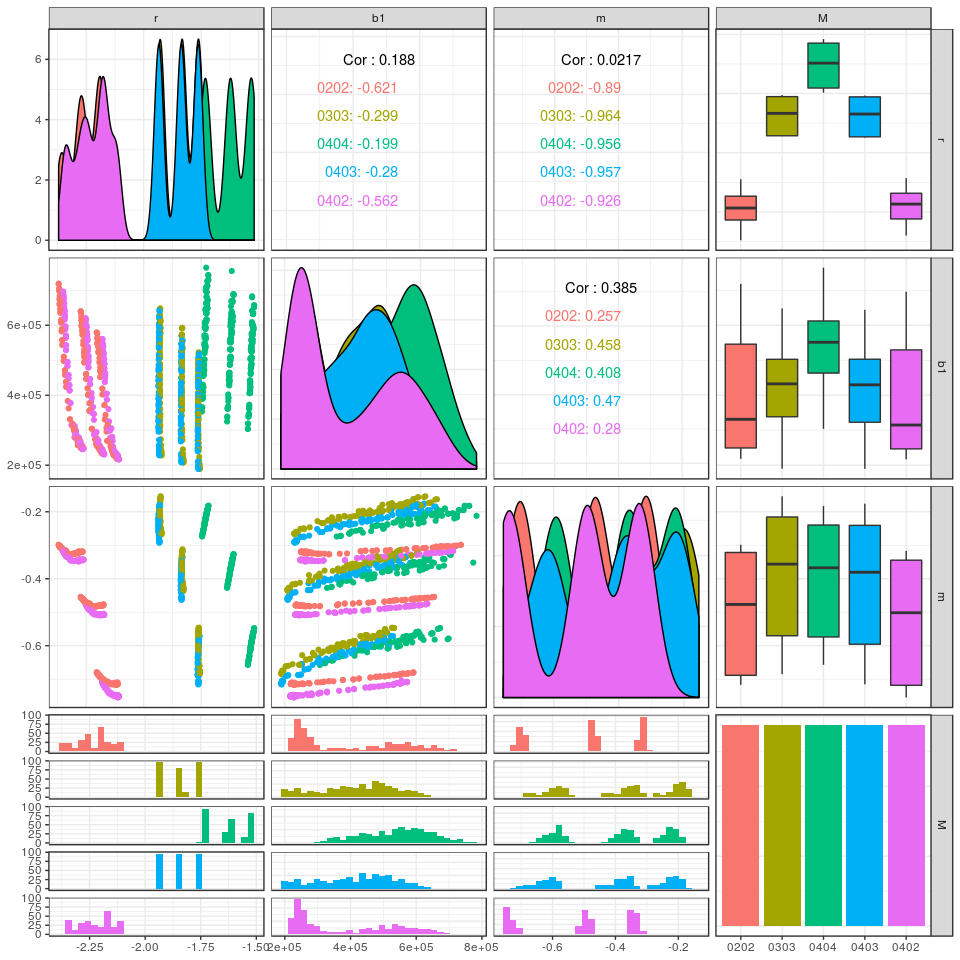
\includegraphics[width=0.75\textwidth]{alb-prior4-1.png}
\caption{\label{fig:grid} Summary of grid scenarios.}
\end{figure}

\begin{figure}[ht!]
\centering
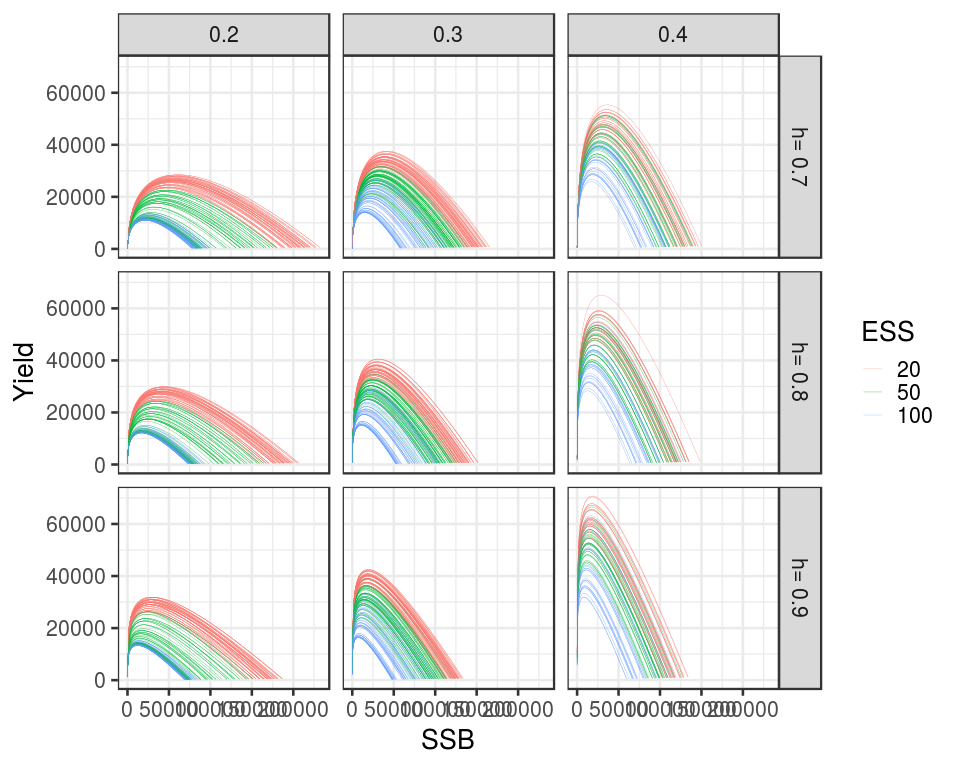
\includegraphics[width=0.75\textwidth]{alb-pfunc-1.png}
\caption{\label{fig:pf} Production functions for the full grid.}
\end{figure}

\begin{figure}[ht!]
\centering
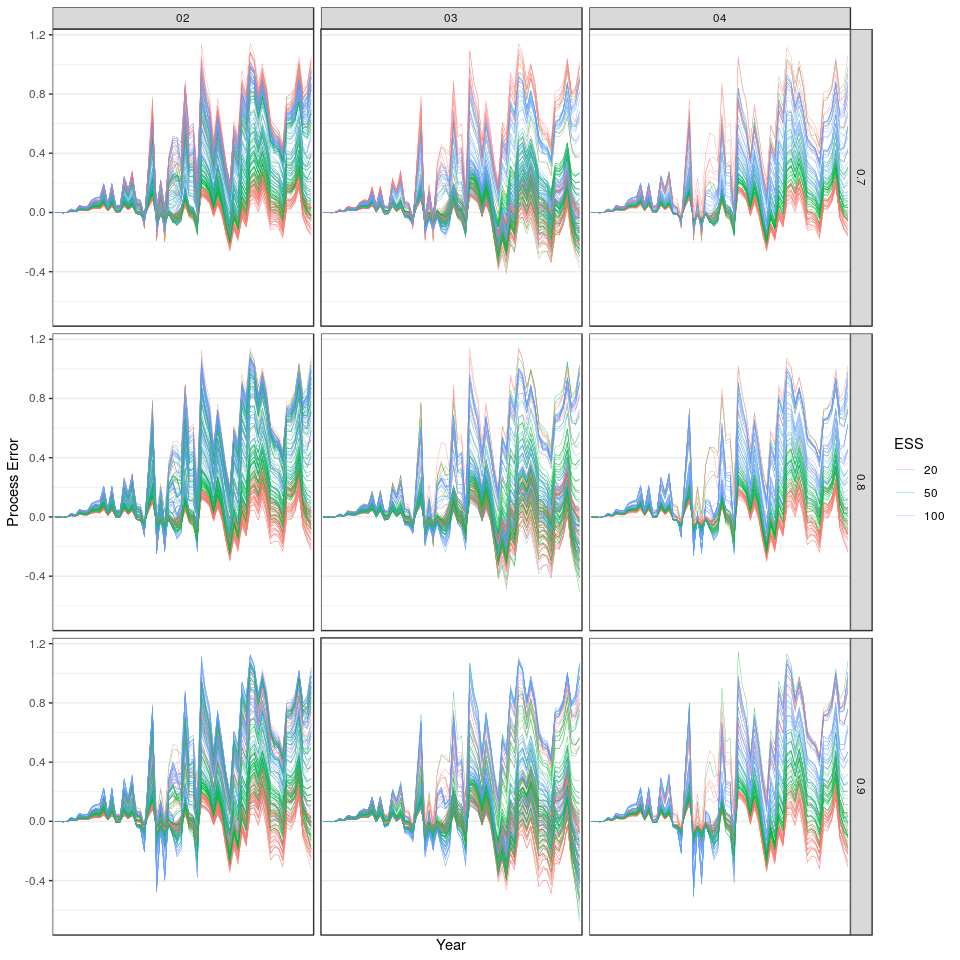
\includegraphics[width=0.75\textwidth]{alb-pe-1.png}
\caption{\label{fig:pe} Process error for the full grid.}
\end{figure}


\end{document}


\subsection{How to include Figures}

First you have to upload the image file from your computer using the upload link the project menu. Then use the includegraphics command to include it in your document. Use the figure environment and the caption command to add a number and a caption to your figure. See the code for Figure \ref{fig:frog} in this section for an example.

\subsection{How to add Comments}

Comments can be added to your project by clicking on the comment icon in the toolbar above. % * <john.hammersley@gmail.com> 2016-07-03T09:54:16.211Z:
%
% Here's an example comment!
%
To reply to a comment, simply click the reply button in the lower right corner of the comment, and you can close them when you're done.

Comments can also be added to the margins of the compiled PDF using the todo command\todo{Here's a comment in the margin!}, as shown in the example on the right. You can also add inline comments:

\todo[inline, color=green!40]{This is an inline comment.}

\subsection{How to add Tables}

Use the table and tabular commands for basic tables --- see Table~\ref{tab:widgets}, for example. 

\begin{table}
\centering
\begin{tabular}{l|r}
Item & Quantity \\\hline
Widgets & 42 \\
Gadgets & 13
\end{tabular}
\caption{\label{tab:widgets}An example table.}
\end{table}

\subsection{How to write Mathematics}

\LaTeX{} is great at typesetting mathematics. Let $X_1, X_2, \ldots, X_n$ be a sequence of independent and identically distributed random variables with $\text{E}[X_i] = \mu$ and $\text{Var}[X_i] = \sigma^2 < \infty$, and let
\[S_n = \frac{X_1 + X_2 + \cdots + X_n}{n}
      = \frac{1}{n}\sum_{i}^{n} X_i\]
denote their mean. Then as $n$ approaches infinity, the random variables $\sqrt{n}(S_n - \mu)$ converge in distribution to a normal $\mathcal{N}(0, \sigma^2)$.


\subsection{How to create Sections and Subsections}

Use section and subsections to organize your document. Simply use the section and subsection buttons in the toolbar to create them, and we'll handle all the formatting and numbering automatically.

\subsection{How to add Lists}

You can make lists with automatic numbering \dots

\begin{enumerate}
\item Like this,
\item and like this.
\end{enumerate}
\dots or bullet points \dots
\begin{itemize}
\item Like this,
\item and like this.
\end{itemize}

\subsection{How to add Citations and a References List}

You can upload a \verb|.bib| file containing your BibTeX entries, created with JabRef; or import your \href{https://www.overleaf.com/blog/184}{Mendeley}, CiteULike or Zotero library as a \verb|.bib| file. You can then cite entries from it, like this: \cite{greenwade93}. Just remember to specify a bibliography style, as well as the filename of the \verb|.bib|.

You can find a \href{https://www.overleaf.com/help/97-how-to-include-a-bibliography-using-bibtex}{video tutorial here} to learn more about BibTeX.

We hope you find Overleaf useful, and please let us know if you have any feedback using the help menu above --- or use the contact form at \url{https://www.overleaf.com/contact}!
